\documentclass[11pt]{article}

\usepackage[english]{babel}                 %% hyphenation rules, spell-checker
\usepackage{amsmath}                        %% macros like align* and pmatrix
\usepackage{graphicx,epstopdf}              %% for .eps graphs
\usepackage[official]{eurosym}              %% 1 \euro
\usepackage[a4paper,margin=2cm]{geometry}   %% margins

\frenchspacing                              %% no extra space after period
\addtolength{\parskip}{0.5\baselineskip}    %% some white space between paragraphs
\setlength{\parindent}{0pt}                 %% but no indentation
\renewcommand{\baselinestretch}{1.1}        %% line spacing of TeX is small

\title{Non-life --- Assignment X}  %% don't forget to change!

\author{
  Y\footnote{Student number: 00000000}
  \quad and \quad
  Z\footnote{Student number: 99999999}
}

\date{\today}

\begin{document}

\maketitle

\subsection*{Question 1}

The power of \LaTeX~lies in easy and beautiful typesetting of complicated formulas like
\[
   \sum_{n=0}^\infty x^n = \frac{1}{1-x},
\]
or
\[
   \int_{-\pi}^{\pi} \sin \left(\frac{x}{2}+\pi\right) \text{d}x = 0,
\]
or
\[
  \begin{pmatrix}
    1 & 2 & 3 \\ %% \\ denotes `next row/line'; & denotes `next column'
    4 & 5 & 6
  \end{pmatrix}
  \begin{pmatrix}
    1 \\ 1 \\ 1
  \end{pmatrix}
  =
  \begin{pmatrix}
    6 \\ 15
  \end{pmatrix}.
\]

In an \verb!align*! environment (included in package \verb!amsmath!) the characters following the tab-sign \& are aligned:
\begin{align*}
  ( 1 - x ) ( 1 + x + x^2 + \ldots + x^n )
  & = 
  1 - x + x - x^2 + x^2 - \ldots + x^n - x^{n+1}
  \\ %% denotes `next line'
  & =
  1 - x^{n+1}.
\end{align*}


\subsection*{Question 2}

The \verb!verbatim! environment serves to typeset source code, or output, of programs:

\begin{verbatim}
> X <- c(100, 120, 80, 80, 120)
> mean(X); sd(X)
[1] 100
[1] 20
\end{verbatim}

\newpage %% new page, if you think that's necessary
\subsection*{Question 3}

%%To insert an R-graph into your document, save it in encapsulated postscript (.eps) format by right-clicking on it. In RStudio, export it to this format, or just use pdf.
%%Put the following in your LaTeX-file:

A centered graph in encapsulated postscript (.eps) format as produced by R:

\begin{center}
\textbackslash{}includegraphics[scale=.6]{IG.eps} 
\end{center}

Other file formats like .jpg work as well:

\begin{center}
\textbackslash{}includegraphics[scale=.6]{Poisson.jpg}
\\
Sim\'eon Denis Poisson (21 June 1781 -- 25 April 1840)
\end{center}

\bigskip

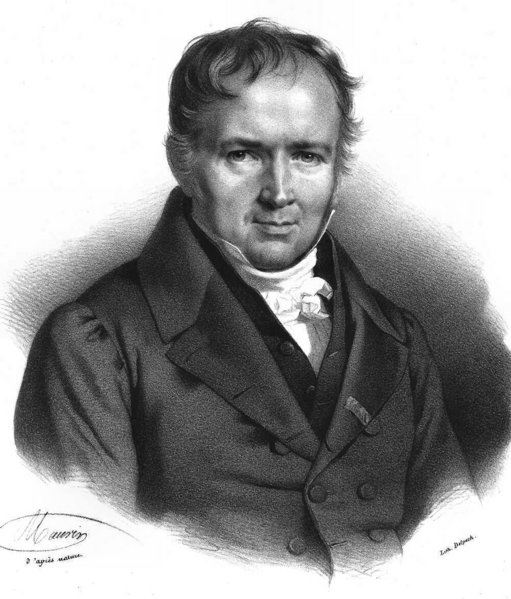
\includegraphics[height=7cm]{Poisson.jpg}

\includegraphics[scale=.4]{GNU.png}

\bigskip 

With and without copyright notice:

\hfill\includegraphics[scale=.4]{ladder1.pdf}\hfill
%trim option's parameter order: left bottom right top
\includegraphics[trim = 0mm 0mm 5mm 0mm, clip, scale=.4]{ladder1.pdf}\hfill\mbox{}


\end{document}
